\subsection{Mögliche Datengrundlage und Format}
\label{sub:mögliche_datengrundlage_und_format}
  Für eine Visualisierung von Öffentlichen Verkehrsmittel wären mehrere Ansätze denkbar. Einige davon sollen nachfolgend beschrieben werden.

  \subsubsection{Einsatz von GPS-Daten}
  \label{ssub:einsatz_von_gps_daten}
    Eine Möglichkeit ist eine GPS-basierte Visualisierung der Echtzeitpositionen der Vehicle. Dies ist eine exakte Abbildung des momentanen Zustandes des Verkehrsnetzes und entspricht am ehesten einer Abbildung des realen "`Ist"'-Zustands. Die einzelnen Vehicle würden in einem festen Intervall von n-Sekunden ihre Position senden, welche sich dann auf einer Karte anzeigen ließe. Je nach Frequenz des Aktualisierungsintervalls, wäre das Ergebnis der Position genauer oder ungenauer.

    Der Einstaz von GPS hat aber allerlei Schwachstellen, die auf den ersten Blick vielleicht nicht offensichtlich sind.

    \begin{itemize}[label={}]
      \item \textbf{Fehlende Datenverfügbarkeit:}
        Ein Weg, um Echtzeitdaten zu visualisieren, wäre die Verarbeitung von GPS-Daten, die von den jeweiligen Verkehrsverbünden zur Verfügung gestellt werden müssten. Dies ist allerdings nicht der Fall. Zwar gibt es durchaus eine Erfassung der Öffentlichen Verkehrsmittel, allerdings werden diese nicht für Dritte zur Verfügung gestellt. Die HaCon GmbH sammelt beispielsweise solche Daten, indem sie diese durch in den Fahrzeugen integrierte Software berechnet.\parencite{havasBusradar}. Es wären also GPS-Daten vorhanden, da sie unter anderem im Bus-Radar der Deutschen Bahn (entwickelt von HaCon) verwendet werden, sie sind allerdings weder über eine API noch anderweitig für die Öffentlichkeit erhältlich. Über die rechtlichen Belange und ob solche Daten in Deutschland überhaupt öffentlich gemacht werden dürften, soll an dieser Stelle nicht diskutiert werden\footnote{In \textit{"`Opening Public Transit Data in Germany"'} von Stefan Kaufmann\parencite{kaufmann} wird dieses Thema der Rechtslage näher betrachtet.}.

      \item \textbf{Aktualisierungsintervall:}
        Abseits der fehlenden Beschaffung von GPS-Daten haben diese noch einen weiteren Nachteil. Vehicle, die mit einer GPS-Lokalisierung ausgestattet sind, senden keinen kontinuierlichen Strom an Daten, sondern nur in einem gewissen Aktualisierungsintervall. Zwar preist HaCon seinen Busradar durch folgende Aussage an: 

        \begin{quote}
          \textit{"`Der neue Busradar eignet sich hervorragend, um die eigene Fahrt zu visualisieren und Anschlussfahrzeuge zu verfolgen. Erstmals geschieht dies GPS-basiert und nicht durch interpolierte Echtzeitdaten, was eine noch höhere Genauigkeit zur Folge hat."'}\parencite{havasBusradar}
        \end{quote}

        Nähme man aber nur die GPS-Daten als Basis für eine Visualisierung, so würde der Bus bei jeder Aktualisierung von der jeweils vorherigen Position zur nächsten springen. Dieses "`Springen"' kann beim Busradar dann auch dazu führen, dass der Nutzer einen Bus auf seiner App verfolgen will, aber dieser nach dem nächsten GPS-Update nicht mehr auf dem Display zu sehen ist, da er nun außerhalb des Viewports liegt. Dieses Verhalten kann den Nutzer durchaus verwirren, da nicht klar ist, in welche Richtung sich das Vehicle bewegt hat, sodass in alle Richtung gesucht werden muss.

      \item \textbf{Verlässlichkeit \& Verfügbarkeit:} 
        Zudem sind GPS-Signale nicht immer verlässlich. Sie können oftmals gestört werden oder die Verbindung zum Satelliten verlieren. Wie würde sich in einem solchen Fall des Signalverlusts die Live-Visualisierung verhalten? Verschwindet das Vehicle von der Karte oder bleibt es für längere Zeit auf der Stelle stehen? Beide Möglichkeiten erscheinen als nicht optimal. 

        Zuletzt sei erwähnt, dass ein GPS-basiertes System für U- und S-Bahn erst gar nicht infrage käme, da diese unterirdisch verlaufen und andere Technologien für deren Erfassung eingesetzt werden müssten. Für eine Live-Karte, die nicht nur Busse, sondern auch andere Verkehrsmittel abbilden möchte, ist die GPS-basierte Lokalisierung folglich nicht zielführend. 

        % (FLEET MANAGEMENT ?)Für Unternehmen allerdings kann eine Visualisierung der eigenen Fleets über die privaten GPS Daten   Eine Visualisierung im Fleet-Management allerdings 
    \end{itemize} 

  % subsection einsatz_von_gps_daten (end)

    \subsubsection{GTFS-Fahrplandaten}
    \label{ssub:gtfs_fahrplandaten}
      Das GTFS (General Transit Feed Specification) ist eine Datenstandardisierung, die von Google im Jahr 2006 entwickelt wurde. Vor dessen Einführung gab es weder eine einheitliche Standardisierung, noch ein "`de facto Standard"' für die Fahrpläne des Öffentlichen Nahverkehrs in den USA. Unter anderem aus diesem Grund erfolge die Adaption an das neue GTFS-Format sehr schnell. Vor allem für digitale Produkte, wie zum Beispiel Trip-Planer, die viele verschiedene Fahrpläne von unterschiedlichen Unternehmen in ihren Service integrieren müssen, ist ein standardisiertes Datenformat unbedingt notwendig. Heute sind die meisten öffentlich verfügbaren Fahrpläne im GTFS-Format auf Plattformen wie: \url{http://transitfeeds.com} oder \url{https://transit.land/} frei verfügbar.\footnote{Momentan besitzt Transitfeeds 535 Feeds (Stand 18.08.2017)}. GTFS ermöglichte es Transit Organisationen, ihre Daten für Dritte zu öffnen und ist heute das weit verbreitetste offene Datenformat für den Öffentlichen Nahverkehr\footnote{Dies gilt allerdings nicht für Deutschland, hier bieten zum jetzigen Zeitpunkt nur 3 Verkehrsunternehmen ein öffentliches GTFS-Feed an}.\parencite[S. 2]{roush}\\

      Ein GTFS-Feed besteht aus mindestens 6 und maximal 13 \texttt{csv-Dateien}, die im \texttt{.txt} Format vorliegen müssen. Die Struktur eines Feeds lässt sich in Worten wie folgt beschreiben:

      \begin{quote}
        \textit{Ein GTFS-Feed besteht aus einer oder mehreren Routen. Jede Route (\texttt{routes.txt}) hat einen oder mehrere Trips (\texttt{trips.txt}). Jeder Trip besucht eine Abfolge von Stops (\texttt{stops.txt}) zu einer bestimmten Zeit (\texttt{stop\_times.txt}). Trips und Stop-Zeit beinhalten nur die Tageszeitinformationen. Der Kalender (calendar.txt und \texttt{calendar\_dates.txt}) bestimmt dann, an welchen Tagen ein bestimmter Trip stattfindet.} \cite[S. 8]{zervaas}
      \end{quote}

      Um sich den Inhalt einer GTFS-Datei besser vorstellen zu können, ist nachfolgend ein Auszug der \texttt{stops.txt} Tabelle abgebildet.

      \begin{lstlisting}[captionpos=b, caption=Auszug der ersten Zeilen von \texttt{stops.txt}, label=lst:gtfs-auszug]
        stop_id,stop_name,stop_lat,stop_lon
        668,Moetzingen Bruehlstrasse,48.53249,8.775416
        2840,Ludwigsburg Mainzer Allee,48.9018,9.21601
        6409,Burgholzhof,48.81742,9.191285
      \end{lstlisting}

      Nachfolgend sind kurz die wichtigsten Tabellen beschrieben.

      \begin{itemize}
        \item \texttt{agency.txt} beinhaltet Informationen über die Verkehrsunternehmen, welche das Feed und die Daten bereitstellen.

        \item \texttt{routes.txt}: Eine Route ist eine Gruppierung von Trips. Die verschiedenen Eigenschaften einer Route werden in dieser Tabelle gespeichert.

        \item \texttt{trips.txt}: Ein Trip gehört zu einer Route. Eine Route kann dabei beliebig viele Trips haben. Welche Trips aktiv sind, wird durch den Kalender festgelegt.

        \item \texttt{calendar.txt} bestimmt, an welchen Tagen ein Trip aktiv ist.

        \item \texttt{stop\_times.txt}: Diese Tabelle beschreibt, welche Stationen nacheinander angefahren werden. Für jede Station beinhaltet sie die Ankunfts- und Abfahrtszeiten.

        \item \texttt{stops.txt} stellt nähere Informationen für jede Station zur Verfügung wie zum Beispiel den Stationsnamen und deren Position.

        \item \texttt{shapes.txt}: Jeder Trip hat eine dazugehörigen Polyline.

      \end{itemize}

      Ein UML-Diagramm, welches die in Relation stehenden Dateien aufzeigt, existiert unter folgender Adresse: \url{https://developers.google.com/transit/gtfs/reference/} 

      \subsubsection*{Fehlende Echtzeitkomponente}
      \label{ssub:fehlende_echtzeitkomponente}
        Aber auch GTFS besitzt Nachteile. Für eine Live-Visualisierung fehlt ihr die Echtzeitkomponente. Die Fahrplandaten stellen nur einen \texttt{Soll-Zustand} dar, der erheblich vom \texttt{Ist-Zustand} abweichen kann. Die reale Position eines Vehicles kann somit nicht wiedergegeben werden, da die tatsächliche Verkehrslage nicht berücksichtigt wird. Dies wirkt sich besonders dann nachteilig aus, wenn Verkehrsmittel sich aufgrund von Staus oder sonstigen Verzögerungen verspäten, Verkehrsmittel ganz ausfallen oder aufgrund von Baustellen etc. umgeleitet werden müssen. Solche außerfahrplanmäßigen Vorkommnisse kann die Visualisierung ohne Echtzeitkomponente nicht bewältigen.
        Auch die Geschwindigkeit eines Vehicles entspricht bei einer Interpolation lediglich der Durchschnittsgeschwindigkeit, die sich anhand der Fahrplandaten ausrechnen lässt. Benötigt ein Vehicle $V$ von Station A nach B 3 Minuten für eine Strecke von 1.2 Kilometer, so würde die Animation eine durchschnittliche Geschwindigkeit von $v = \frac{s}{t} = \frac{1.2 \: \cdot \: 1000}{3 \: \cdot \: 60} = 6.6 \: \frac{m}{s} = 23.76 \: \frac{km}{h}$ errechnen. Diese kann zwar in vielen Fällen wie bspw. dem Schienen- oder Überlandsverkehr zutreffen, berücksichtigt aber im Stadtverkehr weder Geschwindigkeitsbegrenzungen noch Wartezeiten an Kreuzungen. 

      % ssub:fehlende_echtzeitkomponente (end)

      \subsubsection*{Uneinheitliche Gestaltung von GTFS}
      \label{ssub:uneinheitliche_gestaltung_von_gtfs}
        Trotz der Standardisierung durch GTFS gibt es immer noch diverse Freiräume in der Umsetzung des Formats. Wie anfangs erwähnt wurde, beträgt die Anzahl der Dateien, die für ein gültiges GTFS-Feed benötigt werden, nur 6. Es sind allerdings bis zu 13 Dateien möglich. Dies zeigt, wie viele unterschiedliche Informationen ein GTFS Feed bereitstellen kann, aber nicht muss. 
        Auch innerhalb der Dateien gibt es Felder, die vorhanden sein "`müssen"' oder nur "`dürfen"'. Beispielsweise muss das Feld \texttt{route\_short\_name} in \texttt{routes.txt} vorhanden sein, aber \texttt{route\_desc} (Route Description) nicht. Der Interpretationsspielraum lässt sich aber noch weiter veranschaulichen, wenn wir uns Tabelle ~\ref{table:gtfs_differences} ansehen. In dieser Tabelle sind zwei Einträge aus unterschiedlichen GTFS Feeds aufgelistet.
        Wir sehen, dass die Spalte \texttt{route\_id} bei Stuttgart-VVS als Zahlenwert angegeben wird, wohingegen Boston-MBTA einen Text verwendet.

        \begin{longtable}{|>{\raggedright \arraybackslash}p{3.0cm}|>{\raggedright \arraybackslash}p{2.0cm}|>{\raggedright \arraybackslash}p{3.5cm}|>{\raggedright \arraybackslash}p{5.5cm}|}
        \caption{Unterschiede innerhalb GTFS} 
        \label{table:gtfs_differences}\\
          \hline
           & route\_id & route\_short\_name & route\_long\_name\\
          \hline
          Stuttgart-VVS & 379 & U1 & Fellbach - Hauptbahnhof - Vaihingen\\
          \hline
          Boston-MBTA & Blue Line & Blue & Bowdoin - Wonderland\\
          \hline
        \end{longtable}

        "`Blue Line"' ist dabei die Bezeichnung der U-Bahnlinie\parencite{wiki_blue_line}. Wir sehen also, dass Stuttgart-VVS die \texttt{route\_id} zur eindeutigen Identifizierung mittels Zahlenwert verwendet, wohingegen Boston-MBTA dieses Feld nutzt, um den Namen der Linie zu beschreiben. Angenommen, wir verwenden die \texttt{route\_id} in einer Benutzeroberfläche wie in Abbildung~\ref{fig:gtfs_differences}.

        \begin{figure}[htbp]
          \begin{center}
            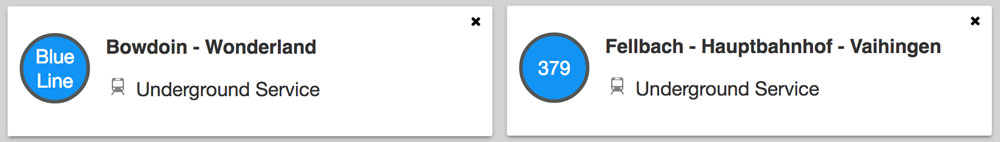
\includegraphics[width=\textwidth]{gtfs_differences.jpg}
            \caption{UI Element mit GTFS Informationen}
            \label{fig:gtfs_differences}
          \end{center}
        \end{figure}

        Links in der Abbildung ist die korrekte Bezeichnung der Route zu sehen, nämlich \texttt{Blue Line}, wohingegen rechts nur eine numerische ID zu sehen ist, die nicht für den Nutzer vorgesehen und damit falsch ist. Damit die rechte Seite korrekt wäre, müsste dort \texttt{U1} abgebildet sein. Die fehlende, beziehungsweise nicht gegebene Übereinstimmung der beiden Feeds führt also zu Problemen bei der Darstellung, die auch durch die Verwendung eines anderen Feldes wie zum Beispiel \texttt{route\_short\_name} nicht behoben werden können. 

        Dies ist nur ein Beispiel, bei dem Abweichungen in der Ausführung der Spezifikation, eine Auswirkung auf die Programmierung haben. Aus diesem Grund ist im März 2017 auf \url{http://gtfs.org/} eine neue \texttt{Best-Practices} Sektion erschienen. Dabei handelt es sich um Empfehlungen an die Hersteller von GTFS Feeds, um eine Verwendung der Feeds möglichst zu vereinheitlichen. Würden sich alle Hersteller an solch eine striktere Implementierung der Spezifikation halten, müssten Programmierer weniger "`Edge Cases"'\footnotemark abfangen und Anwendungen würden in Qualität und Zuverlässigkeit noch besser werden.\\

        \footnotetext{Ein "`Edge Case"' ist ein Problem oder eine Situation, die nur bei einem extremen (maximalen oder minimalen) Betriebsparameter auftritt.}

        \subsection*{Probleme beim Auslesen von Daten}
        \label{sub:subsection_name}
        % subsection subsection_name (end)
        Ein weiteres Problem in GTFS ist das Auslesen von Daten. GTFS lässt sich zwar sehr einfach in eine relationale Datenbank überführen, aber das Auslesen der Daten kann schnell sehr komplex werden, sodass die Geschwindigkeit für eine Webanwendung nicht mehr schnell genug ist. Bereits 1993 stellte \texttt{Jakob Nielsen} einen Richtwert für die responsive Wahrnehmung einer Webanwendung vor:

        \begin{quote}
          \textit{"`1.0 second is about the limit for the user's flow of thought to stay uninterrupted, even though the user will notice the delay. Normally, no special feedback is necessary during delays of more than 0.1 but less than 1.0 second, but the user does lose the feeling of operating directly on the data."'}\parencite{nielsen}
        \end{quote}

        Ob oder wie die Geschwindigkeit erreicht werden kann, soll hier nicht vertieft werden, denn diesem Thema habe ich bereits meine Bachelorarbeit gewidmet\parencite{lorer}.

        Damit eine Webanwendung aber überhaupt eine Chance hat, diese Geschwindigkeitsmarke zu erreichen, ist eine schnelle Antwortzeit des Backends sehr wichtig. Dabei sind Antwortzeiten innerhalb von 1 bis 200 Millisekunden ein sehr guter Wert. Natürlich gilt: Je weniger umso besser.\\

        Das GTFS Format hat den entscheidenden Nachteil, dass es eine hohe Komplexität aufweist, sobald Daten aus verschiedenen Tabellen benötigt werden. Für eine Live-Visualisierung, sind Daten aus nahezu allen Tabellen relevant. Abbildung \ref{fig:gtfs_joined_tables} zeigt, welche davon benötigt - beziehungsweise nicht benötigt werden (grau).

        \begin{figure}[htbp]
          \begin{center}
            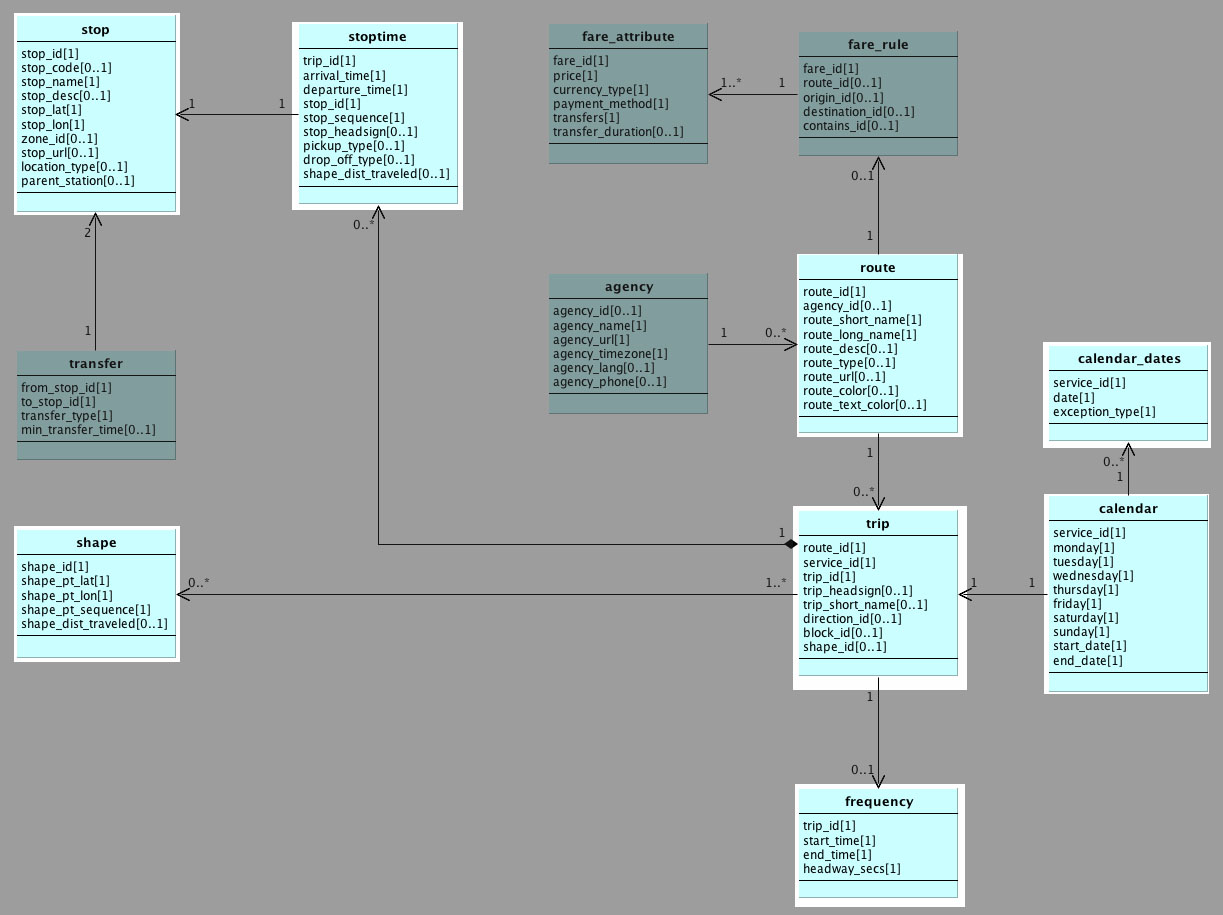
\includegraphics[width=0.85\textwidth]{gtfs_joined_tables.jpg}
            \caption{Benötigte GTFS Tabellen\parencite{google_gtfs_reference}}
            \label{fig:gtfs_joined_tables}
          \end{center}
        \end{figure}

        Das UML Diagramm ist auf den ersten Blick relativ simpel zu verstehen und die Grundlagen der verschiedenen Relationen wurde bereits in Kapitel \ref{ssub:gtfs_fahrplandaten} beschrieben. Wo liegt also das Problem? In Worten ließe sich diese Datenbankabfrage mit folgendem Statement beschreiben: 

        \begin{quote}
          \label{query_statement}
          \textit{"`Gib uns alle aktiven Trips mit deren Linienverlauf, die am heutigen Tag aktiv sind und in einer Zeitspanne zwischen $t_a$ und $t_b$ liegen."'}
        \end{quote}

        Das große Problem dieses Satzes liegt in der Zeitkomponente \textit{"`Trips die am heutigen Tag aktiv sind zwischen ..."'}. Die Trip Tabelle selbst (bezogen auf Abbildung \ref{fig:gtfs_joined_tables}), bietet diesbezüglich keinerlei Informationen. Auch die Calendar- und Calendar-Dates Tabelle beinhaltet nur Informationen darüber, an welchem Datum ein Trip stattfindet, nicht aber um welche Uhrzeit. 

        Erst die Stoptime-Tabelle ermöglicht es uns, eine Aussage zu treffen, wann ein Trip aktiv ist. Über die zwei Felder \texttt{arrival\_time} und \texttt{departure\_time} lässt sich sagen, zu welchem Zeitpunkt ein Vehicle an einer Station anhält. Die erste und letzte Station ($S_1$ und $S_n$) geben uns also einen zeitlichen Rahmen, in dem der Trip aktiv ist.
        Hierbei wird klar, dass allein die Beantwortung der Frage zur zeitlichen Komponente bereits sehr viele Daten aus verschiedenen Tabellen benötigt. Die anderen Tabellen wie \texttt{shape}, \texttt{route}, \texttt{stop} und \texttt{frequency} würden für weitere Informationen wie Vehicle-Farbe, Stop-Position (Längen- und Breitengrad) oder für die Polyline benötigt werden. Um an die Daten zu gelangen, müssen alle relevanten Tabellen mittels SQL \texttt{JOIN} miteinander verknüpft werden. Dies geschieht durch die Verbindung der einzelnen Reihen zweier Tabellen (TabelleA und TabelleB) gegen eine Verknüpfungsbedingung. Das Resultat ist eine neue Ergebnistabelle mit den Inhalten der kombinierten Reihen. Solche Verknüpfungen sind besonders dann zeitintensiv, wenn eine große Menge an Daten (siehe Tabelle: \ref{table:table_metrics}) kombiniert werden. Die Metriken der Tabellen sind dabei wie folgt:

        \begin{longtable}{|>{\raggedright \arraybackslash}p{5.0cm}|>{\raggedright \arraybackslash}p{5.0cm}|>{\raggedright \arraybackslash}p{5.0cm}|}
        \caption{Tabellen Metriken} \label{table:table_metrics}\\
          \hline
          Tabellen Name & Anzahl Reihen\\
          \hline
          trips.txt & 71,000\\
          stop\_times.txt & 1,3000,000\\
          stops.txt & 7,900\\
          shapes.txt & 1,085,860\\
          \hline
        \end{longtable}
        
        Die für das oben genannte Statement \ref{query_statement} äquivalente SQL-Abfrage ist aufgrund seiner Länge (113 Zeilen Code) im Anhang unter Listing \ref{lst:get_active_trips_query} zu finden. Diese SQL Abfrage ist allerdings nicht performant. Sollen alle Trips in einem Zeitraum von 1 - 15 Minuten gefunden werden, sind bereits Rechenzeiten entstanden, die aufgrund ihrer langen Laufzeit abgebrochen werden mussten. In mehreren Iterationen wurde versucht, die SQL-Abfrage zu optimieren, was allerdings keine Verbesserung herbeiführte. Es sind zu viele JOIN Verknüpfungen und WHERE Bedingungen in dieser Abfrage, als dass sich eine performante Lösung damit finden ließe. Es musste ein neuer Ansatz gefunden werden, um Abfragezeiten erheblich zu verringern.
      % subsubsection freiräume_in_der_gestaltung_von_gtfs (end)
    % subsubsection gtfs_fahrplandaten (end)
    
    \subsubsection{GTFS-Realtime}
    \label{ssub:gtfs_realtime}
      Eine andere Möglichkeit für die Erfassung von Echtzeitpositionen und Verspätungen bietet GTFS-realtime. GTFS-realtime ist ein von Google entwickelter Standard, der Verkehrsunternehmen das Bereitstellen von Echtzeitinformationen ermöglicht. Dabei gibt es 3 verschiedene Feeds, die GTFS-realtime zur Verfügung stellt:\parencite{zervaas_realtime}[S. 6]

      1. Vehicle positions\\
      2. Trip updates\\
      3. Service alerts\\

      GTFS-realtime wäre für diese Arbeit deshalb interessant, da diese Spezifikation Updates zu Trips und Vehicle-Positionen ermöglicht. Beispielsweise kann die Interpolation anhand der Verspätung eines Vehicles angepasst werden. Ein Auszug eines Trip-Updates ist in Listing~\ref{lst:gtfs_rt_trip_update} zu sehen.

      \begin{lstlisting}[captionpos=b, caption={Auszug eines GTFS-realtime Trip Updates von MBTA},label={lst:gtfs_rt_trip_update}]
  {
  id: 25732950
  trip_update {
    trip {
      trip_id: 25732950,
      start_date: 20150120,
    }
    stop_time_update {
      arival {
        delay: 240
      }
      stop_id: 135
      ...
    }
    ...
  }
  }
    \end{lstlisting}

    Vehicle-Positionen können über ein ähnliches Format bezogen werden Listing~\ref{lst:gtfs_rt_vehicle_position_update}.

    \begin{lstlisting}[captionpos={b},caption={Auszug eines GTFS-realtime Vehicle-Position Updates von MBTA},label={lst:gtfs_rt_vehicle_position_update}]
  {
  id: "v121",
  vehicle {
    trip {
      trip_id: 2590683,
      start_date: 2017017
    },
    position {
      latitude: 42.267967,
      longitude: -71.093834
    },
    ...
  }
  }
    \end{lstlisting}

  Für eine ausführlichere Beschreibung hilft das Buch: \textit{"`The Definitive Guide to GTFS-realtime - How to consume and produce real-time public transportation data with the GTFS-rt specification."'}\parencite{zervaas_realtime} von Quentin Zervaas.\\

  % subsection gtfs_realtime (end)
% subsection mögliche_datengrundlage_und_format (end)